%%%%%%%%%%%%%%%%%%%%%%%%%%%%%%%%%%%%%%%%%%%%%%%%%%%%%%%%%%%%%%%%%
%  _____       ______   ____									%
% |_   _|     |  ____|/ ____|  Institute of Embedded Systems	%
%   | |  _ __ | |__  | (___    Wireless Group					%
%   | | | '_ \|  __|  \___ \   Zuercher Hochschule Winterthur	%
%  _| |_| | | | |____ ____) |  (University of Applied Sciences)	%
% |_____|_| |_|______|_____/   8401 Winterthur, Switzerland		%
%																%
%%%%%%%%%%%%%%%%%%%%%%%%%%%%%%%%%%%%%%%%%%%%%%%%%%%%%%%%%%%%%%%%%

\chapter{MIDI Steuerung}\label{chap.midi}

\section{Blockschaltbild und Schnittstellen}

Als erstes die Zusammenfassung der internen Blöcke. Die zwei entwickelten Blöcke \textit{midi control} und \textit{polyphonie out} sind grau markiert (siehe Abbildung \ref{fig.midi_interface_block} ). Gegeben ist der Block uart top. \\

\begin{figure}[H]
	\centering
	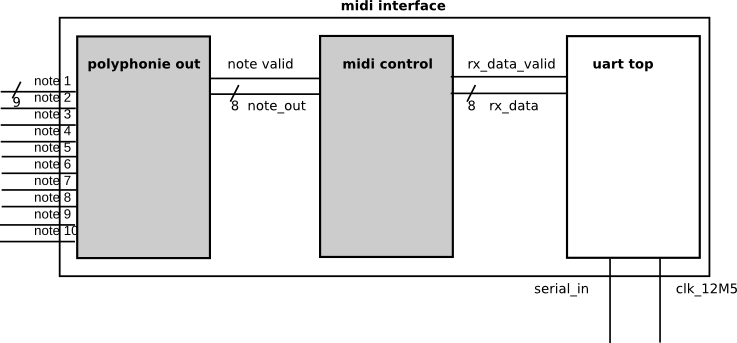
\includegraphics[width=0.7\textwidth]{images/midi_interface/midi_interface_block.png}
	\caption{Blockschaltbild Midi Interface}
	\label{fig.midi_interface_block}
\end{figure}


\textbf{Definition der Schnittstellen}\label{schnittstellen}

\textbf{Uart Top Ausgang}
\begin{itemize}
	\item 8-Bit-Signal: Bytweise Dekodierung der Midi Daten 
	\item 1-Bit-Signal: Übermittelt Gültigkeit der Daten
\end{itemize}

\textbf{Midi Control Ein- und Ausgang}
\begin{itemize}
	\item Empfangen von 8-Bit Midi Daten, \hspace*{20mm}Empfangen, ob Daten korrekt sind (1 Bit)
	\item Übermittelt 9-Bit-Notenvektor (Abb.\ref{fig.Notenvektor}) \hspace*{10mm}Übermitteln, ob Daten korrekt (1 Bit)
\end{itemize}

\textbf{Polyphonie Out Ein- und Ausgang}
\begin{itemize}
	\item Eingang eines 9-Bit-Notenvektors \hspace*{22mm}Eingang, ob Daten gültig sind
	\item Ausgabe von 10 Notenvektoren zu 9-Bit.
\end{itemize}
\bigskip
Im vorgegebenen Konzept für Polyphonie out (siehe Unterkapitel \ref{konzept_plyphonie}) ist die Schnittstelle zum Polyphonie Out-Block als ein 9-Bit-Signal definiert. Das MSB dient als Flag, ob die übermittelte Note an oder ab ist.
\begin{figure}[H]
	\centering
	
\includegraphics[width=0.2\textwidth]{images/midi_interface/NotenVektor.png}
	\caption{Aufbau Notenvektor}
	\label{fig.Notenvektor}
\end{figure}

Als nächstes wird die MIDI 1.0 Spezifikation, erklärt, nach der Block \textit{midi control} aufgebaut ist. Die Umsetzung des \textit{polyphone out}-Blocks bildet den Abschluss dieses Kapitels.\\


\newpage
\section{Das MIDI Kommunikationsprotokoll}\label{sect.midi_spezification}
Werden MIDI Daten übermittelt, so unterscheidet der Standard zwei Typen an Daten \ref{Midi_specification}.

\subsection{MIDI Daten Typen}\label{datenytpen}
\subsubsection*{Status Bytes}
\textit{Status bytes} sind 8 Bit lang und das MSB ist immer logisch '1'.  \textit{Status bytes} dienen dem Identifizerein der nachfolgenden \textit{data bytes}. Das \textit{status byte} definiert die Datenstruktur der folgenden \textit{data bytes}.
\newline
\newline
MIDI behält einen Status, bis ein neues \textit{status byte} folgt. Dieses Verhalten ist als \textit{running status} bezeichnet. Dieses Verhalten ist für Polyphonie relevant, da der Zustand bleibt, bis dass ein neues \textit{status byte} folgt..

\subsubsection*{Data Bytes}
Gemäss Spezifikation folgen einem \textit{status byte} exakt ein oder zwei Bytes. Das MSB ist immer logisch '0'. Die Werte können von 0x00 bis 0x7F sein. Das bedeutet, dass MIDI maximal 128 Noten unterscheiden kann.
\newline
\newline
\textit{Data bytes} können unterschiedliche Informationen erhalten. Im Kontroller sind Notenwerte, Geschwindigkeit des Anschalges relevant
\newline
\newline
Je nachdem \textit{status byte} werden die \textit{data byte} anders interpretiert. 
\newline
\newline
''Empfänger sollen so konzipiert sein, dass zuerst alle\textit{data bytes} empfangen werden und ein neues \textit{status byte} kommt. Danach werden ungültige Daten verworfen. Einzige Ausnahme ist der \textit{running status}. Bei dem nicht bis zum Ende gewartet wird.''\ref{Midi_specification}.\\

\subsubsection*{Ungültige Bytes}
''Alle \textit{status bytes}, die nicht implementierte Funktionen enthalten und alle ihnen folgenden \textit{Data Byte}s sollen vom Empfänger verworfen werden.''\ref{Midi_specification}.\\ MIDI Geräte sollen ausdrücklich beim Ein- und Abstellen darauf bedacht sein, dass keine undefinierten Bytes gesendet werden\ref{Midi_specification}.\\
Diese Anforderung ist wichtig beim Implementieren der \textit{finate state machine} und der \textit{testbench} (siehe \ref{polyphonitest}) \\

\subsubsection*{Midi Bytes binär}\label{midi_binaer}
\begin{itemize}
	\item ''0xxx xxxx'': \hspace*{10mm}Definition \textit{data byte}
	\item ''1xxx xxxx'': \hspace*{10mm}Definition \textit{status byte}		
	\item ''1000 xxxx'': \hspace*{10mm}Definition NOTE OFF
	\item ''1001 xxxx'': \hspace*{10mm}Definition NOTE ON
	\item ''1010 xxxx'': \hspace*{10mm}Definition POLYPHONY
	\item ''100x xxxx'': \hspace*{10mm}Erste drei Bits der \textit{status bytes} NOTE ON (0x90) und NOTE OFF (0x80)
\end{itemize}
%---5.2-----------------------------------------------------------------------
\newpage
\subsection{Zwei MIDI-Noten-Modi}\label{note_modes}
\subsubsection{Datenstruktur}
Die Datenstruktur der zwei MIDI-Noten-Modi beginnt mit dem \textit{status byte} (grau in der Abbildung \ref{fig.testbench_single_Mode}). Es folgt der Notenwert (hier einen Dummy-Wert von 0x11 eingetragen) und die Geschwindigkeit. Letztere hat im \textit{single mode} keine spezfiische Bedeutung, im \textit{polyphony mode} bestimmt die Geschwindigkeit, ob die Note an oder ab ist.\\


\begin{figure}[H]
	\centering
	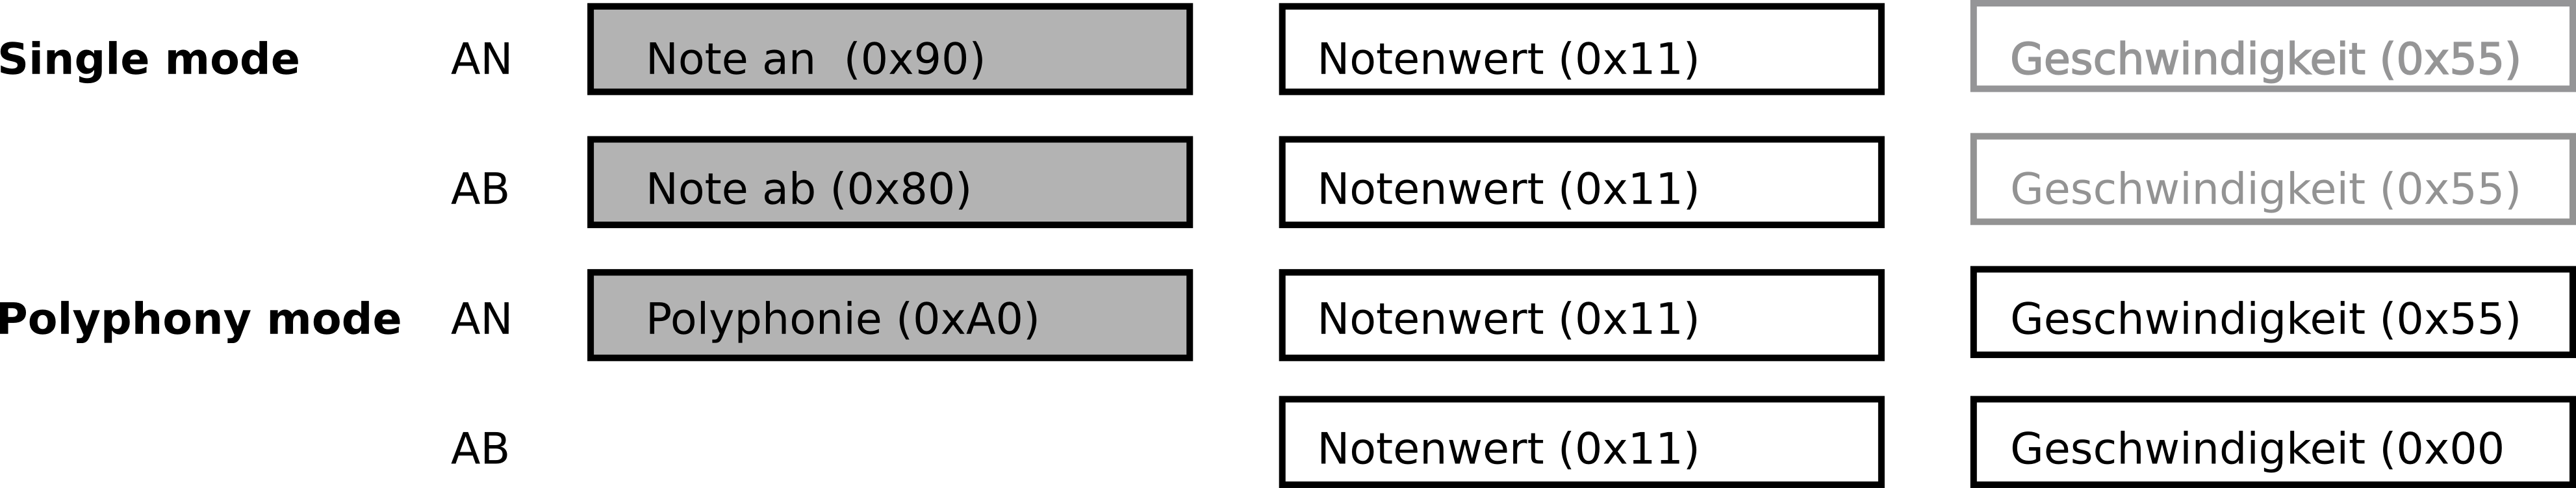
\includegraphics[width=1\textwidth]{images/midi_interface/MIDI_Spezifikation.png}
	\caption{MIDI Spezifikation für Datenstruktur einzelne Note und Polyphonie}
	\label{fig.testbench_single_Mode}
\end{figure}

Unterschiedlich zu behandeln ist die Funktion des \textit{status bytes}. Im \textit{single mode} wird mit dem \textit{status byte} der Zustand an oder ab mitgegeben. Im \textit{polyphony mode} wird nur der Noten-Modus mitgeteilt und das \textit{status byte} hat keine weiteren Funktionalitäten. In der Abbildung wird der Platz von Note an oder ab bezüglich dem Noten-Byte durch graue Markierung veranschaulicht. Die zeitliche Reihenfolge der ist umgekehrt, was in der Token-Verarbeitung berücksichtigt werden muss.\\

\begin{figure}[H]
	\centering
	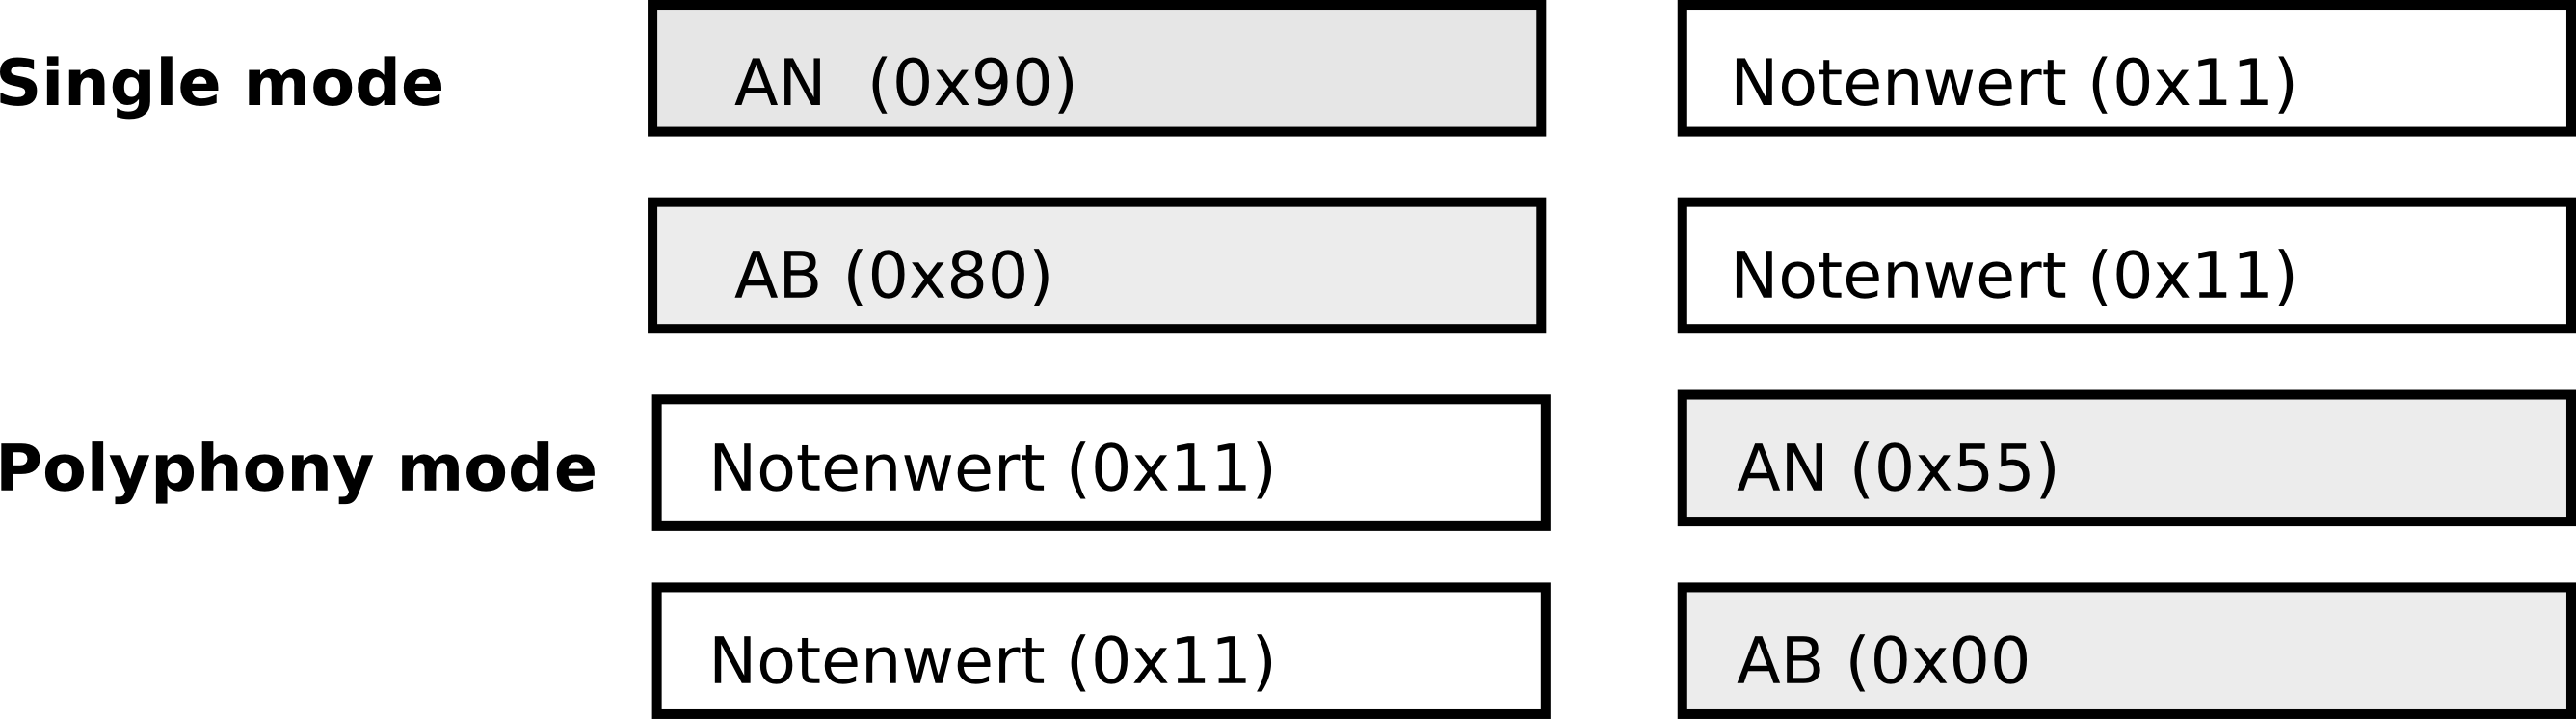
\includegraphics[width=0.7\textwidth]{images/midi_interface/MIDI_Spezifikation_Datenfolge.png}
	\caption{Blockschaltbild Device under Test}
	\label{fig.testbench_polypphon_mode}
\end{figure}

Wegen der unterschiedlichen Bedeutung der eingegangenen Token, behandelt die \textit{fsm} die zwei Noten-Modi und deren Noten- und Geschwindigkeitszustände unabhängig voneinander.



%------5.3-------------------------------------------------------------
\newpage
\section{Umsetzung Midi Control-Block}\label{sect.midi_umsetzung}

\subsection{Anforderung an die Finate State Machine und Skizze}\label{anforderung_fsm}
Der Controller wird über eine \textit{finite state machine} implementiert. Ausgehend von der Spezifikation \ref{sect.midi_spezification} sind drei Eckpunkte berücksichtigt:
\begin{enumerate}
	\item Unterscheiden von \textit{status byte} und \textit{data byte}
	\item Unterschiedliche Interpretation der \textit{data bytes} abhängig vom \textit{status byte}.
	\item Verwerfen aller falschen \textit{status byte} oder \textit{data bytes}
\end{enumerate}
\smallskip
Vereinfacht verhält sich die \textit{fsm} wie in Abbildung \ref{fig.midi_fsm_skizze} gezeigt. 
\begin{figure}[H]
	\centering
	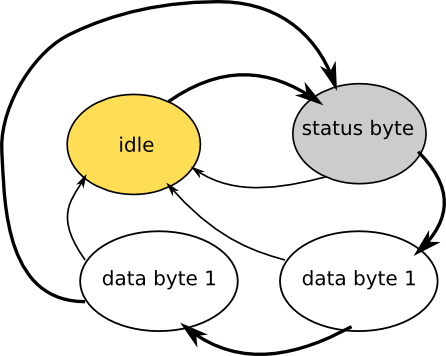
\includegraphics[width=0.3\textwidth]{images/midi_control/fsm_grob_2.png}
	\caption{Skizze der fsm}
	\label{fig.midi_fsm_skizze}
\end{figure}

Startpunkt der Verarbeitung ist das \textit{status byte} (grau hinterlegt). Danach führt die Verarbeitung durch die zwei \textit{data bytes}. \\
In jedem Zustand, werden ungültige Daten verworfen, und führen zurück zu idle. Die Verarbeitung wird fortgesetzt, wenn das nächste \textit{status byt}e folgt.\\
\newline
Nicht angeschrieben sind die Übergangsbedingungen: data\_valid = '1' wechselt zwischen den Zustänen und data\_valid = '0' verbleibt im Zustand. Die breiteren Pfeile heben die fehlerfreie Datenverarbeitung hervor.\\

\subsection{Implementation Finate State Machine}
Aufgrund der unterschiedlichen Datenstruktur für den \textit{polyphony mode} und den \textit{single mode} besitzen beide Noten-Modi ihre eigenen Zustände (siehe Abbildung \ref{fig.midi_fsm_detail}). \\ 
\newline
Die implementierten Zustände sind
\begin{itemize}
	\item idle: \hspace*{19mm}Alle nicht näher spezifizierten Vorfälle verwerfen
	\item single: \hspace*{16mm}Eintreten in  \textit{single mode} durch \textit{status bytes} 0x80 oder 0x90
	\item note\_s: \hspace*{15mm}Erstes \textit{data byte} im  \textit{single mode}
	\item velocity\_s: \hspace*{10mm}Zweites \textit{data byte} im \textit{single mode}
	\item polyphonie: \hspace*{8mm}Eintreten in polyphony mode durch status byte 0xA0
	\item note\_v:  \hspace*{15mm}Erstes \textit{data byte} im  \textit{polyphony mode}
	\item velocity\_v:  \hspace*{10mm}Zweites \textit{data byte} im  \textit{polyphony mode}
\end{itemize}


\newpage
Abbildung \ref{fig.midi_fsm_detail} definiert die Übergangsbedingungen. Drei generelle Verhaltensweisen sind vereinfacht angegeben:

\begin{itemize}
	\item data\_valid = '0'\hspace*{10mm}Im akutellen Zustand bleiben.\\
	 \hspace*{34mm}Dargestellt mit Pfeil an Ort
	\item data\_valid = '1'\hspace*{10mm}Grundbedingung für Zustandswechsel\\
	\hspace*{34mm}Gilt implizit zu jedem Pfeil und dessen Bedingung dazu
	\item data(7) = '1' and (data(7 downto 5) /=''100'' or data(7 downto 4)/= ''1010'') \hspace*{5mm} \\
	\hspace*{34mm}\textit{Status bytes}, die nicht \textit{polyphony} oder \textit{single mode} bedeuten, verworfen\\
	\hspace*{34mm}Dargestellt durch Pfeil oben rechts zu idle. Gilt für jeden Zustand
\end{itemize}
\bigskip

Die Übergangsbedingungen detektiert die Binärstruktur der MIDI Daten, die im Unterkapitel \ref{midi_binaer} aufgelistet ist.


\begin{figure}[H]
	\centering
	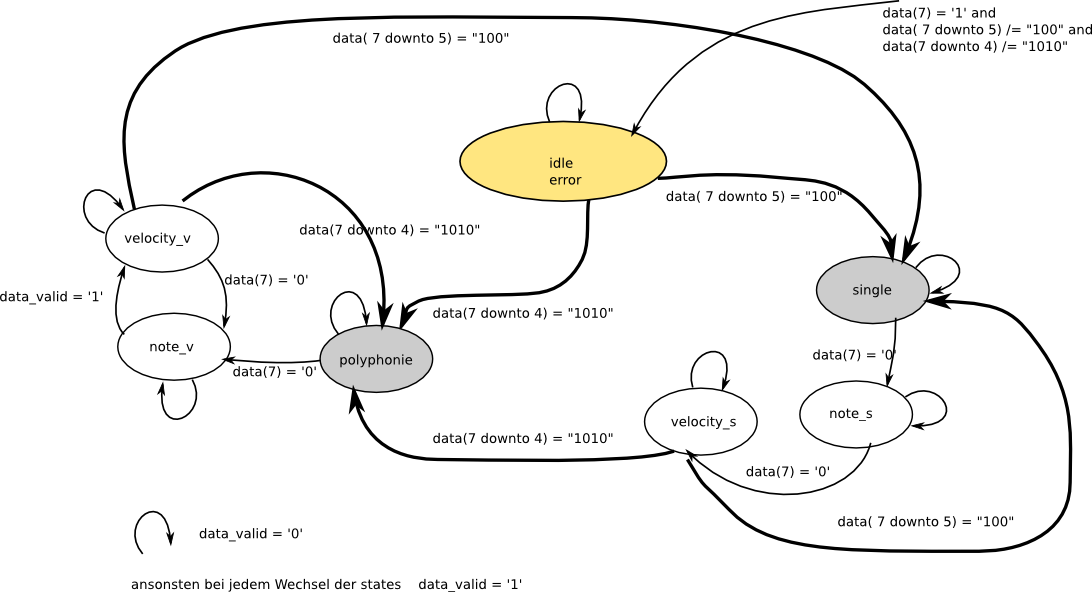
\includegraphics[width=1\textwidth]{images/midi_control/fsm_detailliert.png}
	\caption{Übergänge der fsm}
	\label{fig.midi_fsm_detail}
\end{figure}

Alle drei Anforderungen \ref{anforderung_fsm}, die sich aus der Midi Spezifkation ergeben, sind implementiert:
\begin{enumerate}
	\item Vor jedem \textit{data byte} muss ein \textit{status byte} eingegangen sein. Die \textit{finite state machine} fragt im \textit{idle} Zustand nur nach den \textit{status bytes}. Nach dem \textit{status bytes} erwartet die \textit{finate state machine} \textit{data bytes}. 
	\item Die unterschiedliche Datenstruktur der zwei Noten-Modi ist mode-spefifisch implementiert:\\
Im \textit{single mode} wird das vierte Bit des \textit{status bytes} zum Setzen von an und ab verwendet . \\
Im \textit{polyphony mode} wird das zweite \textit{data byte}, die Geschwindigkeit zum Setzen der Note auf an oder ab verwendet. \\ Geschwindigkeit = NULL ist als Note aus implementiert.\\
	\item Ungültige Bytes sind verworfen, und die \textit{fsm }kehrt in den   \textit{idle} Zustand zurück.
\end{enumerate}


%------5.4------------------------------------------------------------
\newpage
\section{Resultat Midi Control-Block}\label{sect.midi_resultat}

\subsection{Implementierte Finate State Machine}
Das ist die in quartus generierte \textit{fsm} des Blocks \textit{midi control}.
\begin{figure}[H]
	\centering
	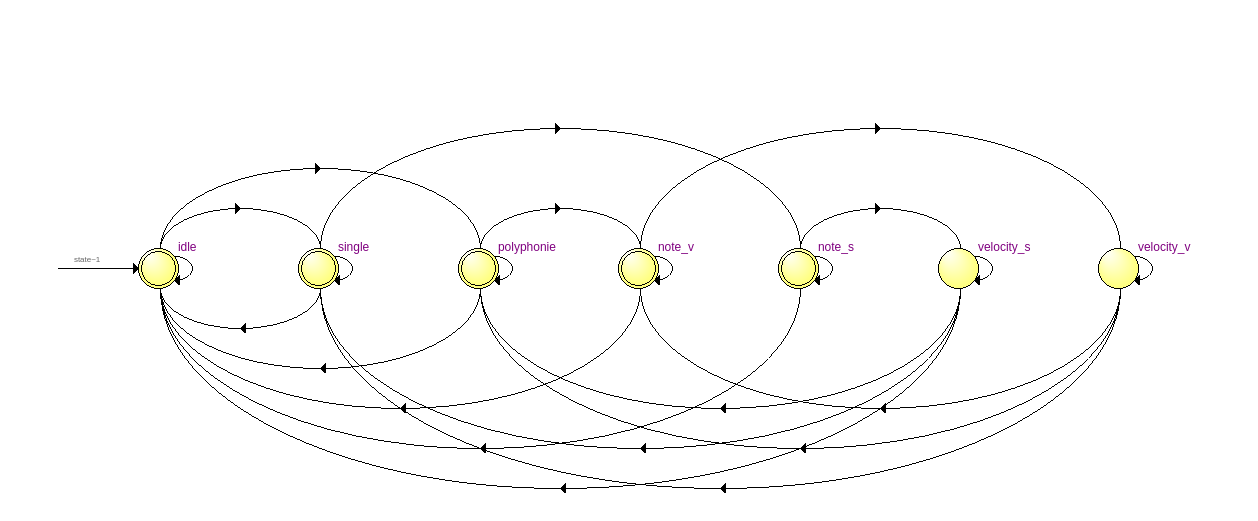
\includegraphics[width=1\textwidth]{images/midi_control/fsm_midicontrol.png}
	\caption{Implementierte fsm im Block Midi Control}
	\label{fig.midi_fsm_quartus_}
\end{figure}


\subsection{Simulation Single Mode}

\textbf{Input Daten} (Zeile 3, siehe Anhang \ref{chap.anhang_midi_input})\\
55 90 27 80 27 90 02 00 00

\textbf{Beschreibung der Befehle}\\
- 55 als Dummy-Velocity für alle Noten\\
- Note an\\
- Notenwert 27\\
- Note ab\\
- Notenwert 27\\
- Note an\\
- Notenwert 02\\
- Dummywerte\\

\textbf{Erwartetes Resultat}\\
Der Kontroller erkennt die Note 27, schaltet diese an und gibt am Ausgang den Vektor ''Note-27-AN'' aus. Dieselbe Note wird nochmals detektiert, diesmal als ab und der Vektor am Ausgang zeigt ''Note-27-AB'' an. Die nächste Note hat den Wert 2 und wird auf AN gesetzt. Der Ausgang gibt ''Note-2-AN'' aus.\\


\newpage

\begin{figure}[H]
	\centering
	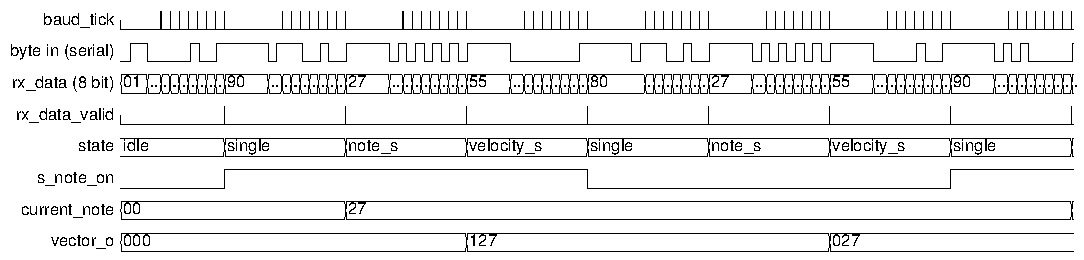
\includegraphics[width=1\textwidth]{images/midi_control/wave_single.png}
	\caption{fsm für single mode}
	\label{fig.midicontrol_singlet}
\end{figure}

\begin{itemize}
	\item Das Signal rx\_data detektiert die Befehle (0x90) und (0x80).
	\item Der Controller interpretiert  \textit{single modus}. 
	\item Die Zustandsabfolge ist korrekt: single, note\_s, velocity\_s.
	\item Zustände werden bei rx\_data\_valid = '1' die Zustände geändert.
\end{itemize}

Die Simulation zeigt, dass die Notenwerte korrekt gespeichert sind und dass das An- und Abstellen der Noten funktioniert. Am Ausgang erscheint der zusammengesetzer Vektor aus den 8 Notenbits und einem vorangestellten Bit, das detektiert, ob die aktuelle Note an oder ab ist. 



\subsection{Simulation Polyphony Mode}
\textbf{Input Daten} (Zeile 11, siehe Anhang \ref{chap.anhang_midi_input})\\
02 55 03 00 20 00 40 55 00

\textbf{Beschreibung der Befehle}\\
- Notenwert 02\\
- Note an\\
- Notenwert 03\\
- Note ab\\
- Notenwert 02\\
- Note ab\\
- Notenwert 40\\
- Note an\\

\textbf{Erwartetes Resultat}\\
Der Kontroller erkennt die Note 02, schaltet diese an und gibt am Ausgang den Vektor ''Note-02-AN'' aus. Die Note 03 wird detektiert, auf ab gesetzt und der Vektor am Ausgang zeigt ''Note-03-AB'' aus. Die nächste Note hat den Wert 2 und wird auf ab gesetzt. Der Ausgang gibt ''Note-2-Ab'' aus. Als letztes folgt die Note 40, die angestellt wird.\\

\begin{figure}[H]
	\centering
	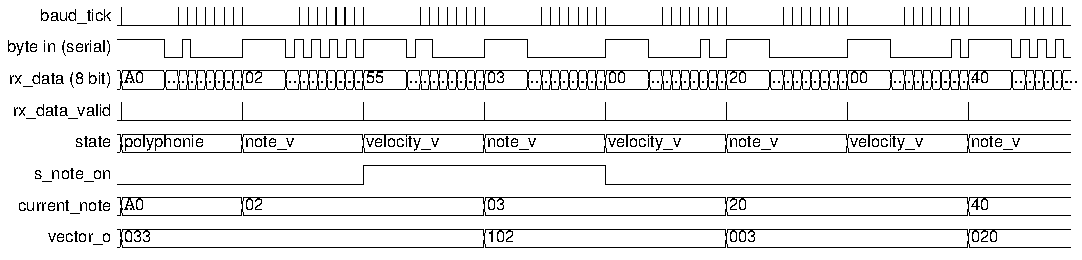
\includegraphics[width=1\textwidth]{images/midi_control/wave_polyphonie.png}
	\caption{fsm im polyphony mode}
	\label{fig.midicontrol_polyphonie}
\end{figure}


\begin{itemize}
	\item Das Signal rx\_data detektiert den Befehle (0xA0).
	\item Der Controller interpretiert  \textit{polyphony mode}. 
	\item Die Zustandsabfolge ist korrekt: polyphonie, note\_v, velocity\_v.
	\item Der Controller wartet mit dem Setzen der Note am Ausgang, bis klar ist, ob die Note an oder ab ist. \\
	Keine kurzfristig falschen Noten am Ausgang, die ab sind.
	\item Zustände werden bei rx\_data\_valid = '1' die Zustände geändert.
	\item Noten können beliebig an- und abgestellt werden
\end{itemize}


\section{Umsetzung Polyphone Out-Block}\label{sect.polyphonie_umsetzung}
 
\subsection{Funktionsbeschreibung}
Der Polyphone Out-Block speichert die empfangenen Signale in 10 Registern. Bei jeder neuen Note wird geprüft, ob der Wert im Register besteht und ob das ON/OFF-Bit der gespeicherten neu gesetzt werden muss. Der Block gibt 10 Noten parallel aus.\\

\begin{figure}[H]
	\centering
	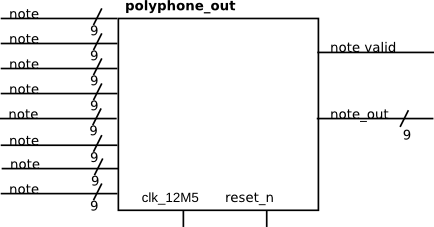
\includegraphics[width=0.5\textwidth]{images/midi_interface/polyphonie_blockschaltbild.png}
	\caption{Polyphone Out-Block}
	\label{fig.polyphnie_out_block}
\end{figure}

\subsection{Konzept}\label{konzept_plyphonie}
Der empfangene Notenwert wird mit den gespeicherten Notenwerten verglichen. Ist eine Note vorhanden, wird das ON-OFF-Bit geprüft und aktualisiert. Keine Note darf zweimal gespeichert sein. Sind alle 10 Registerplätze besetzt, wird die neue Note in ein Register mit abgeschaltenem ON-OFF-Bit gesetzt.\\
\begin{figure}[H]
	\centering
	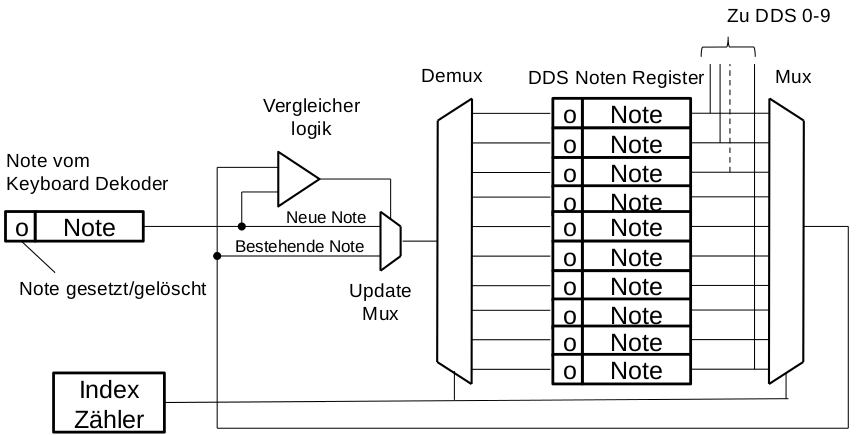
\includegraphics[width=0.7\textwidth]{images/midi_interface/Konzept_Hans_polyphonie.png}
	\caption{Konzept Polyphonie Block \cite{konzept_poly} }
	\label{fig.polyphnie_konzept}
\end{figure}

\subsection{Implementation}
Der Ablauf des Speicherns ist aus der Abbildung \ref{fig.polyphnie_ablauf}.
\begin{figure}[H]
	\centering
	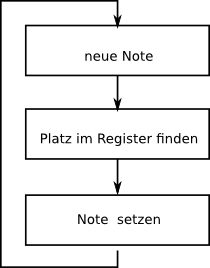
\includegraphics[width=0.2\textwidth]{images/midi_interface/polyphnie_ablauf.png}
	\caption{Ablauf Note speichern }
	\label{fig.polyphnie_ablauf}
\end{figure}

Umgesetz wird das Suchen eines Speicherplatzes innerhalb der 10 Registern mit einer Input-Logik, die mit folgenden 3 Vergleichen arbeitet:
\begin{enumerate}
	\item Liegt der Notenwert in einem Register ? 
	\item Ist ein Register unbenützt ?
	\item Welches Register hat einen abgeschaltenen Notenwert ?
\end{enumerate}
Sobald eine Frage mit Ja beantwortet wird, wird der Registerindex gespeichert und als Output des Logik-Prozesses zur Verarbeitung weiter gegeben.\\
\newline
Durch den übermittelten Index-Wert weiss der Speicher-Prozess, in welches Register die neue Note gespeichert werden soll.\\
Die Werte aller 10 Register werden am Ausgang parallel ausgegeben.



\subsection{Resultat Polyphonie Out-Block}

\begin{figure}[H]
	\centering
	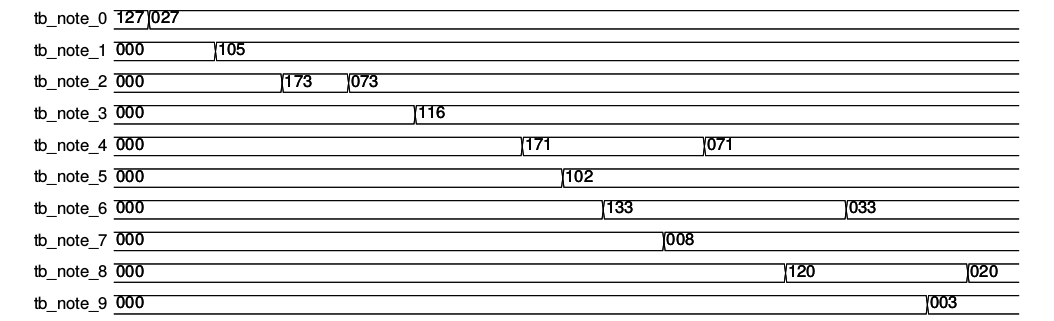
\includegraphics[width=1\textwidth]{images/midi_interface/tb_polyphonie.png}
	\caption{Simulation des Blocks Polyphonie Out }
	\label{fig.polyphnie_simulation}
\end{figure}